\section{Method}
\label{sec:background}

%\begin{center}
%  \smartdiagramset{border color=none, 
%    uniform color list=teal!60 for 4 items,
%  }
%  \smartdiagram[flow diagram:horizontal]{}
%\end{center}

%\begin{tikzpicture}[node distance = 2cm, auto]
%  % Place nodes
%  \node  (init) {$x[n]$};
%  \node [block, right of=init](dnnv) {DNN vocals} ;
%  \node [block, below of=dnnv](dnnb) {DNN bass} ;
%  \node [block, below of=dnnb](dnnd) {DNN drums} ;
%  \node [block, below of=dnnd](dnno) {DNN other} ;
%  \node [right of=dnnv](outv) {$\hat{s}_{vocals}[n]$} ;
%  \node [right of=dnnb](outb) {$\hat{s}_{bass}[n]$} ;
%  \node [right of=dnnd](outd) {$\hat{s}_{drums}[n]$} ;
%  \node [right of=dnno](outo) {$\hat{s}_{other}[n]$} ;
%
%  % Draw edges
%  \path [line, bend left] (init) -- (dnnv);
%  \path [line, bend left] (init) -- (dnnb);
%  \path [line] (init) -- (dnnd);
%  \path [line] (init) -- (dnno);
%  \path [line] (dnnv) -- (outv);
%  \path [line] (dnnb) -- (outb);
%  \path [line] (dnnd) -- (outd);
%  \path [line] (dnno) -- (outo);
%\end{tikzpicture}

\begin{figure}
  \centering
  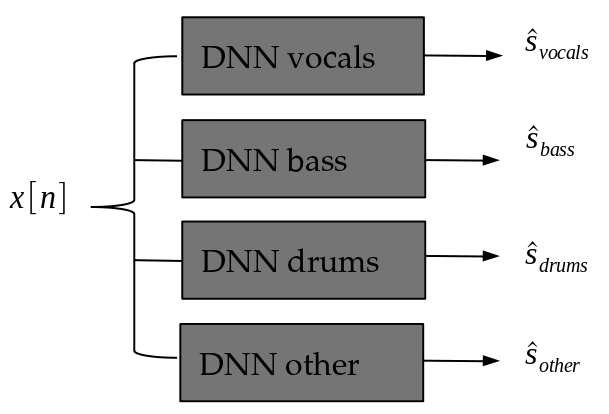
\includegraphics[width=0.5\columnwidth]{mss-basic.png}
  \label{fig:mss-basic}
  \caption{DNN could predict music sources sample per sample}
\end{figure}

In this Section, we present how DNNs are able to solve the music source separation challenge, as in the Figure~\ref{fig:mss-basic}. One naive approach is to use a neural network to predict the estimated source $\hat{s}$ given a sample of the mixture signal $x[n]$. It is noticeable that this simple structure is not using any relation between each samples from $x$. 

Unfortunately, training such neural networks appear particularly difficult. 
Even for human beings, it is impossible to distinguish any pattern on only one sample without any context.
To bring more context to the neural network, the DNN could be fed with a sequence of samples $(x[n+i])_{i\in [-N, N]}$.
Music patterns, such as fading, last of roughly 5 seconds. With a sample rate of 44.1 kHz, the sequence would have a length of $441k$ samples. 
At that size, the curse of dimensionalityi~\cite{mallat} makes it difficult to learn patterns.

%The neural network can not find the invariances between each instruments.

\subsection{Short-term Fourier transform}

Instead, it seems preferable to help the neural network to figure out some invariances using pre-processing steps. 
A widely employed in audio consists in transforming an audio signal into the short-term Fourier transform (STFT). The STFT is a collection of Fourier transform on short section of a signal (typically of 20 ms). The STFT is particularly employed in audio processing, as the signal decomposition is varying around the time axis. 
The STFT is directly derived from the Fourier transform by employing a window function and a delay function:

$$\mathbf{STFT}{x(t)}(\tau,\omega) = X(\tau,\omega) = e^{j\omega t/2}\int_{-\infty}^\infty {x(t)w(t-\tau)e^(-jwt)dt}.$$

Thereafter, we use a Gaussian window function:

$$h(t) = \lambda^{-1/2}\pi^{-1/4}e^{-t^2/(2\lambda^2)}.$$

The STFT of a signal is then a two dimension and complex signal:
$$X(\omega, \tau) = A(\omega, \tau) e^{j\phi(\omega, \tau)},$$
with $\phi$ and $A$ the phase and the amplitude.


\begin{figure}
  \centering
  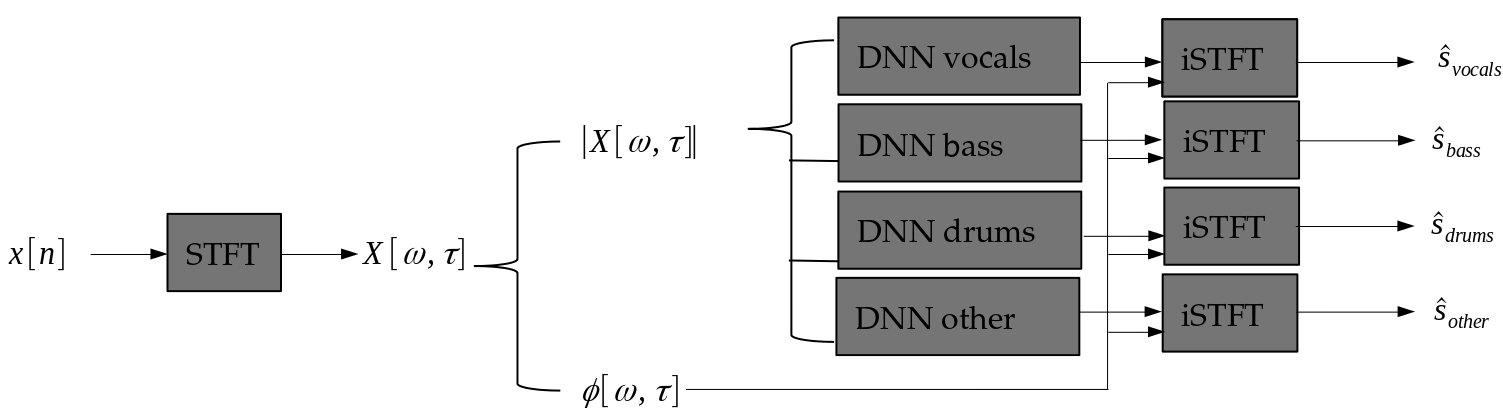
\includegraphics[width=0.9\columnwidth]{mss-amp.png}
  \label{fig:mss-amp}
  \caption{Samples are pre-processed with STFT to ease the appearance of invariances}
\end{figure}

Using an STFT, one solution is to fed the DNN with the amplitude and the phase of the mixture signal, as illustrated in Figure~\ref{fig:mss-amp}.
In this case, the DNN predict the amplitude and the phase of each source. Then the inverse STFT (iSTFT) is applied on the predicted amplitude and phase to reconstruct the source. 


\subsection{Sharing the phase of the mixture signal}

\begin{figure}
  \centering
  \includegraphis[width=0.9\columnwidth]{approx-phase.png}
  \label{fig:approx-phase.png}
  \caption{Comparison between the voice source, the signal reconstructed after an STFT transformation, the signal reconstructed with the phase of the mixture, and with the phase of the drums source}

Predicting the phase is difficult because of its intrinsic discontinuous shape. 
In the context of music source separation, it is generally assumed~\cite{chandna2017monoaural}, \cite{jansson2017singing} that the phase of the mixture signal is the same than each source's phase.
This approximated is illustrated in Figure~\cite{fig:approx-phase}. 

One could wander what is the impact of such transformations on the signal. By computing the signal-to-distortion ratio (SDR), defined as the ratio between the reconstructed signal's power and the original source's power, I observed a loss of 


\subsection{Relations between phase and amplitude} 

The assumption of a Gaussian window allows us to draw a relation between the phase and the amplitude thanks to the work of \cite{auger2012phase}:

\begin{equation}
    [
    \left\{ 
        \begin{array}{ll}
            \frac{\partial }{\partial t}\phi(\omega, \tau) &= \lambda^{-2}   \frac{\partial}{\partial \omega} \log(A(\omega, \tau)) + \frac{\omega}{2} \\
            \frac{\partial d}{\partial \omega}\phi(\omega, \tau) &= -\lambda^{-2}   \frac{\partial}{\partial t} \log(A(\omega, \tau)) - \frac{t}{2}
        \end{array}
    \right.
    ]
\end{equation}

Actually, similar expressions exist for higher order derivatives and for any window function having a certain regularity. 
This relationship provides the intuition to the authors that the derivative of the phase might help a neural network to predict the amplitude.
At the same time, neural networks have stronger difficulties to learn a model when the inputs are correlated.
That is why, 


\subsection{In the discrete time scale}

Numerical audio samples are discretized for discrete time steps $n$, and in this case:
$$\mathbf {STFT} \{x[n]\}(m,\omega ) = X(m,\omega )=e^{j\omega t/2}\sum _{n=-\infty }^{\infty }x[n]w[n-m]e^{-j\omega n}.$$

The intuition of using features extracted from derivatives of the phase required to approximate the discrete time derivatives using finite differences. Thereafter, we use:

$$\Delta_\tau \phi(k, m) = \phi(k, m) - \phi(k,m-1)$$
$$\Delta_\omega \phi(k, m) = \phi(k, m) - \phi(k-1,m)$$



\subsection{Pre-processing}

Pre-processing is used in neural networks to help an optimization algorithm to find symmetries in the training set. Pre-processing is all the more important when the dataset is small. 

In the article of Muth et al., the processing consists in computing the finite-difference derivative and then fixes shits on their distribution.

The authors observed that the distributions of $\Delta_\tau \phi$ and $\Delta_\omega \phi$ are illustrated in Figure~\ref{fig:dist-phi}. We observe that $\Delta_\omega \phi$ has a systematic shift of $\pi$, whereas $\Delta_\tau \phi$ has a shift of $2\pi k\frac{n_0}{N}$, where $n_0$ is the hop size, namely the number of taps between two samples $k$ and $k+1$.

The shift of $\Delta_\tau \phi$ is explained by the shift theorem of the discrete Fourier transform \cite{smith2007mathematics}:
$$x(n-n_0) \xrightarrow{\text{DFT}}
e^{j\frac{2\pi}{N}kn_0}X(k).$$

\subsection{Predicting the amplitude with a neural network}

